% Une ligne commentaire débute par le caractère « % »

\documentclass[a4paper]{article}

% Options possibles : 10pt, 11pt, 12pt (taille de la fonte)
%                     oneside, twoside (recto simple, recto-verso)
%                     draft, final (stade de développement)

\usepackage[utf8]{inputenc}   % LaTeX, comprends les accents !
\usepackage[T1]{fontenc}      % Police contenant les caractères français
\usepackage[francais]{babel}
\usepackage{fullpage}
\usepackage{multicol}
\usepackage{hyperref}
\hypersetup{
    colorlinks=true,
    linkcolor=blue,
    filecolor=magenta,      
    urlcolor=red
    }
\usepackage{bookmark}
\usepackage{blindtext}
\setlength\columnsep{30pt}
\usepackage{algorithm2e}
\SetKwComment{Comment}{/* }{ */}
\RestyleAlgo{ruled}


\usepackage{graphicx}  % pour inclure des images
\graphicspath{ {rapport/img/} }

%\pagestyle{headings}        % Pour mettre des entêtes avec les titres
                              % des sections en haut de page

\title{  TP2 : Compréhension des programmes\\Évolution et restructuration des logiciels}
\author{Mohamad Satea Almallouhi \and Tony Nguyen}
\date{10 novembre 2024}



\begin{document}
    \maketitle
    \begin{center}
        % 
\includegraphics[height=.95\textwidth]{logo}
        
\includegraphics[width=\textwidth]{logo}
    \end{center}

    \begin{abstract}     % Résumé du travail
      \emph{Rapport d'exercice sur l'analyse d'un programme par l'analyse statique et de la notion de couplage afin d'en déduire des modules}
    \end{abstract}
    \newpage
    %\dominitoc  % initializer les minitoc
    \tableofcontents
    \listofalgorithms
    \section*{Introduction}
            \addcontentsline{toc}{section}{Introduction}
            \paragraph{}
                Dans le cadre de l'Unité d'Enseignement Évolution et restructuration des logiciels, nous allons analysés un programme en observant son code source de manière statique. L'étape d'extraction des informations a été réalisé précédement. Nous nous trouvons à présent dans l'étape de traitement des propriétés dans le workflow. Nous allons étudier le concept de couplage des classes.

                Tout d'abord, à partir du travail précédent, nous allons nous servir du graph d'appel des méthodes écrites dans les classes du projet analysé. Cela nous permettra de calculer le couplage entre les différentes classes.

                Ainsi, grâce au graph de couplage, nous allons partitioné notre ensemble de classes en différent modules.
        \section*{Démonstration vidéo}
            \addcontentsline{toc}{section}{Démonstration}
            \paragraph{}
                En ligne sur Youtube, à l'adresse URL 
                \url{https://youtu.be/4WYid4mVgWk} 
                une démonstration vidéo de notre travail.
        \section*{Installation}
            \addcontentsline{toc}{section}{Installation}
            \paragraph{}
                Vous trouverez les instructions dans le README.md

    \newpage
    \begin{multicols}{2}
        [
            To Do
            \begin{itemize}
                \item expliqué la solution implémenté
                \item add code picture 
                \item add resultat picture
                \item diagram class visiteur
                \item diagram class de l'app
                \item definition du couplage avec écritures math DONE
                \item tous les algo en latex stylé DONE
                \item → !!! → vidéo ← !!! ← 
            \end{itemize}
            Faire une vidéo, le rapport avec des screenshot des résultats et du code et enfin un read.md(instruction). En plus, pour le bonus, faire une belle application, des tests unitaires, faire le rapport en Latex.
        ]
        \section{UML (juste pour montrer l'organisation)}
        \noindent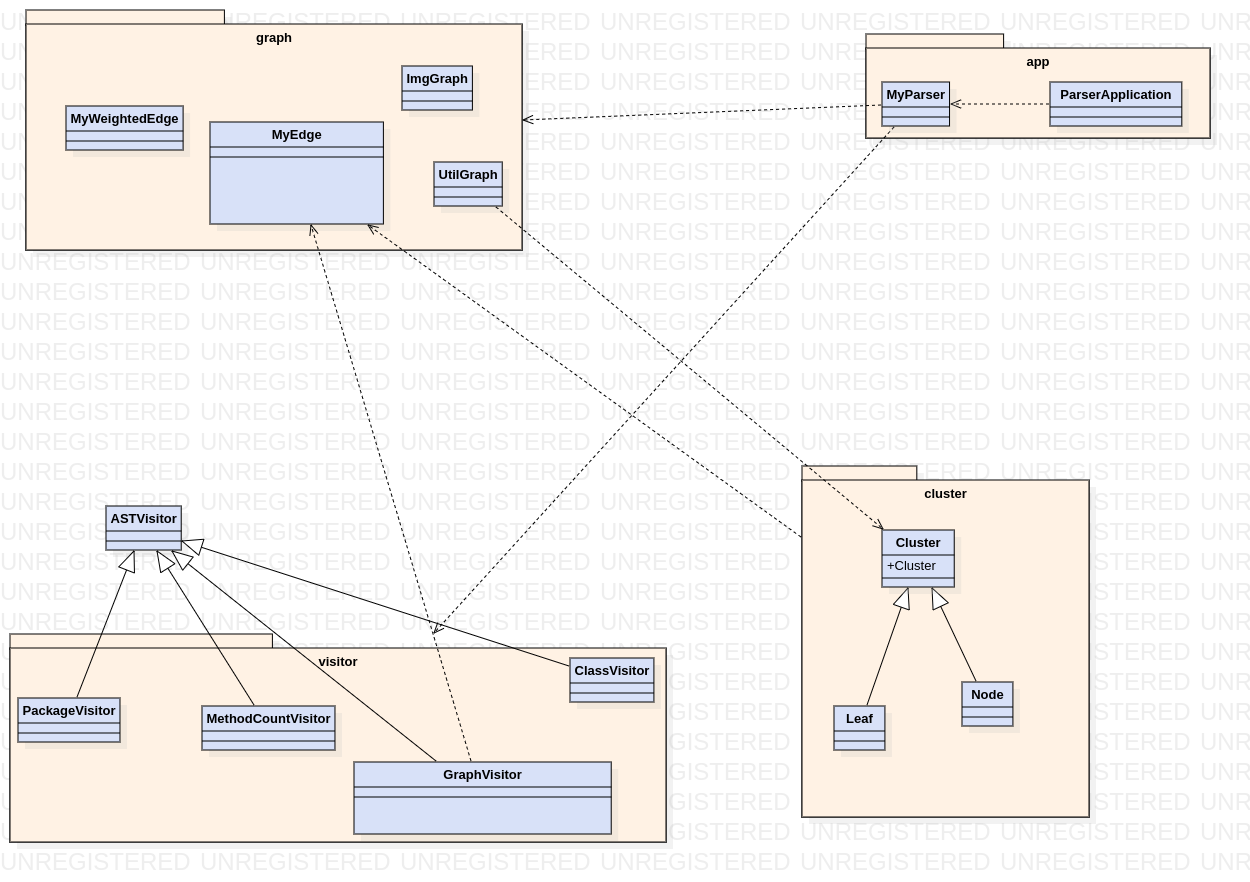
\includegraphics[width=.46\textwidth]{diagram}
        \section{Graphes}
        \paragraph{} 
        Nous nous intéressons au couplage entre les classes de notre application. Il serait logique de réunir les classes fortement dépendantes les unes des autres. De la même façon, les classes qui n'ont aucun rapport entre elle, pour des raisons de clarté, peuvent être isolé.
        \subsection{Algorithmes de création du graphe d'appel}
        \paragraph{} La construction de ce graph est la base de ce travail. Il nous permettra ensuite de calculer le couplage entre les classes ...
        \includegraphics[height=.585\textwidth]{appel/code}
        \paragraph{}
        Lors du parcours de l'arbre syntaxique abstrait (AST), quand on atterit sur un noeud qui correspond à une méthod, on ajoute un noeud au graph et si il y a une méthode invoqué interne au projet, on l'ajoute au graph et on crée une arête.

        Les méthodes qui se surchage entre elles (les méthodes ayant le même nom dans une classe mais avec une signature différente) sont confondues.

        L'algorithme n°\ref{alg:appel} décrivant cela se trouvre à la page \pageref{alg:appel} 

        \paragraph{Résultat} Nous obtenous ainsi le graph suivant :

        \noindent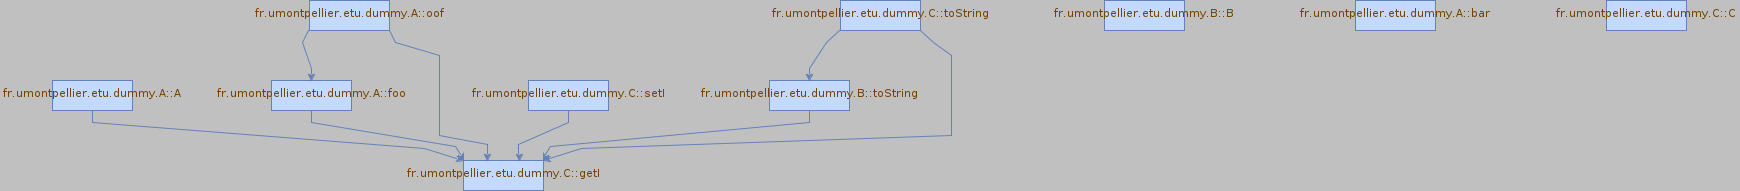
\includegraphics[width=.7\textwidth]{appel/graphAppelShort}
        \subsection{Le couplage}
        \paragraph{Définition} Étant donné une application composé de n classes. Le nombre de méthode d'une classe est noté nbMethod.
        \\
        \\
        \begin{math}
            nbMethodTotal = \sum_{i=0}^n nbMethod_{i}
        \end{math}
        \\
        \\
        \begin{math}
            nbRelationBinaire = nbMethodTotal*nbMethodTotal
        \end{math}
        \\
        \\
        \begin{math}
            nbRelation_{A->B} \neq nbRelation_{B->A}
        \end{math}
        \\
        \\
        \begin{math}
            nbRelation(A,B) = nbRelation_{A->B} + nbRelation_{B->A}
        \end{math}
        \\
        \\
        \begin{math}
            Couplage(A,B) = nbRelation(A,B) / nbRelationBinaire
        \end{math}
        \subsection{Graphe de couplage inter-classes}

        \paragraph{} À partir du graph d'appel, nous allons maintenant créer le graph pondéré par le couplage entre les différentes classes.

        \paragraph{Explication} Pour cela, nous allons créer un graph pondéré où les sommet seront les class et les arête auront un poid égal au couplage entre les class.

        L'algorithme n°\ref{alg:coupling} décrivant cela se trouvre à la page \pageref{alg:coupling} 
        
        \noindent\includegraphics[width=.46\textwidth]{coupl/codeA}
        \noindent\includegraphics[width=.46\textwidth]{coupl/codeB}
        \noindent\includegraphics[width=.46\textwidth]{coupl/codeC}

        \paragraph{} Remarquons que le graph d'appel nous aide à calculer le couplage.

        Par la suite, le graphe pondéré de couplage entre les classes ne sera pas exploité, seul le graph d'appel sera utilisé.

        \paragraph{Résultat} Nous obtenous ainsi le graph suivant :

        \noindent\includegraphics[width=.46\textwidth]{coupl/graphPondereCouplageClass}
        % \subsection{Montrer les visiteur}
        % ???
        \section{Clusturing}
        Nous allons maintenant voir comment nous avons rassemblé les classes entre elles. 
        \subsection{Algorithme de clustering}
        Rassemblons les classes les plus proches entre elles à l'aide du couplage et créons un arbre dendrogramme
        \paragraph{Cluster} L'algorithme n°\ref{alg:dendro} décrivant cela se trouvre à la page \pageref{alg:dendro} avec l'implémentation en java :
        \\\\
        \noindent\includegraphics[width=.46\textwidth]{cluster/codeA}
        \noindent\includegraphics[width=.46\textwidth]{cluster/codeB}
        \noindent\includegraphics[width=.46\textwidth]{cluster/codeC}

        \paragraph{Remarque} Nous utilisons uniquement nbRelation(A,B) et non pas Couplage(A,B). De plus, A et B représente ici un ensemble de class.
        \subsection{Identification des modules / partitionnement des classes}

        \paragraph{Cluster} L'algorithme n°\ref{alg:dendro} décrivant cela se trouvre à la page \pageref{alg:dendro}.

        \noindent\includegraphics[width=.46\textwidth]{module/code}
        \noindent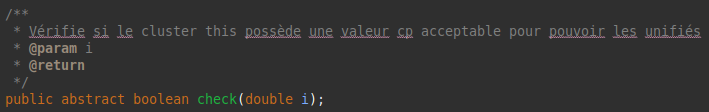
\includegraphics[width=.46\textwidth]{module/check}
        \noindent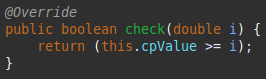
\includegraphics[width=.46\textwidth]{module/checkNode}
        \noindent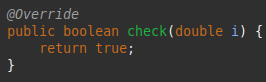
\includegraphics[width=.46\textwidth]{module/checkLeaf}
        % Essayons maintenant de séparer les différentes branches du dendrogramme. Les différentes branches du dendrogramme représente des clusters de class sémentiquement lié. Ces clusters seront nos modules 
        % \paragraph{Partitionnement des classes}
        \section{Spoon}
        \paragraph{} L'un des problème rencontrer est de trouver un moyen pour savoir si une méthode est interne ou externe au programme.

        La solution que nous avons trouvé est de comparer avec le package de la class où la méthode est déclarée.

        \paragraph{} On remarque que le résultat différe entre Spoon et jdt.core.dom.AST. C'est due au fait que Spoon n'a capturé les constructeurs comme des méthodes. Si on regarde les graph d'appel, ils sont identique à l'exception des constructeurs.

        \noindent\includegraphics[width=.46\textwidth]{spoon/code}
        \noindent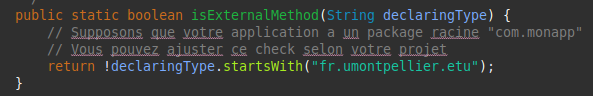
\includegraphics[width=.46\textwidth]{spoon/isExternalMethod}
        \noindent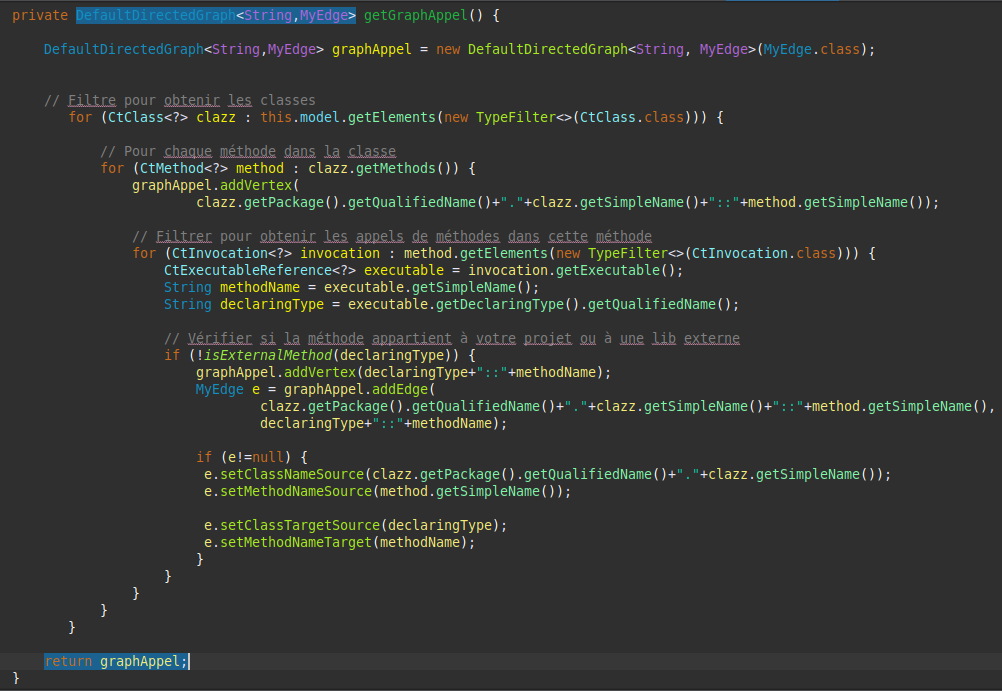
\includegraphics[width=.46\textwidth]{spoon/getGraphAppel}
        \noindent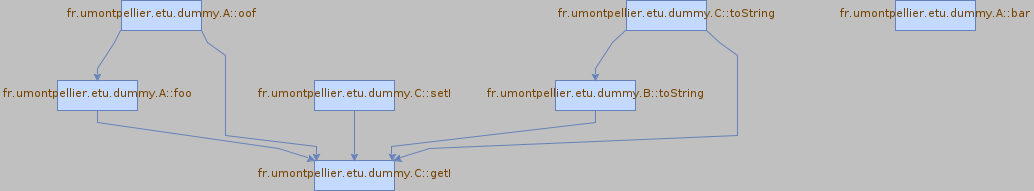
\includegraphics[width=.46\textwidth]{spoon/graphAppel}
        \noindent\includegraphics[width=.46\textwidth]{spoon/graphPondereCouplageClass}
    \end{multicols}

\begin{algorithm}
\caption{An algorithm to make call graph}\label{alg:appel}
\KwData{$programme$}
\KwResult{$graphe\ d'appel$}
$g \gets new\ Graph() $\;
\For{each class c}{
    \For{each method m implemented in c}{
        \For{each method invoqued i in m}{
            \If{!isExternalMethod(i)} {
                $g.addSommet(m)$\;
                $g.addSommet(i)$
                \Comment*[r]{ajout des sommets m et i}

                $g.addVertex(m,i)$ \Comment*[r]{ajoute une arete de m vers i}

            }
        }
    }
}
$return\ g$\;
\end{algorithm}
\begin{algorithm}
\caption{An algorithm to make a weighted graph corresponding to the coupling between class}\label{alg:coupling}
\KwData{$le\ graphe\ d'appel$}
\KwResult{$graphe\ pondere$}
$graphPondere \gets new\ GraphPondere() $\;
\Comment{Produit cartésion entre toutes les classes de l'application en retirant les couples identiques (x,x)}
\For{each String aClassName1 in classNameSet}{
    \For{each String aClassName2 in classNameSet}{
        \If{aClassName1 != aClassName2} {

            $cpValue \gets calculCouplageValueEntre(aClassName1, aClassName2)$\;

            \If{cpValue > 0} {
                $graphPondere.addArete(aClassName1,aClassName2,cpValue)$\;
            }
        }
    }
    }
    $return\ graphPondere$\;
\end{algorithm}
\begin{algorithm}
    \paragraph{UML} INSERT UML CLASS DIAGRAM OF Cluster composite pattern
\caption{Clustering algorithm (Creating the Dendrogramme)}\label{alg:dendro}
\KwData{$graph\ d'appel$}
\KwResult{$the\ dendrogramme$}
\Comment{Stratégie: toutes les class sont leurs propres cluster. On va essayer de fusioner les clusters entre eux en fonction du couplage}
$clusters \gets Cluster[]$\;
\For{each String aClassName in classNameSet}{
    $clusters.add(new\ Leaf(aClassName))$\;
}
$i \gets 0$\;
$Node root \gets null$\;
\While{i < size(clusters)} {
    $n \gets laFusionEntreLes2CLustersLesPlusProche()$\;
    $on\ retire\ les\ 2\ enfants\ du\ noeud\ n$\;
    $clusters.add(n)$\;
    $i++$\;
}
$return\ root$\;
\end{algorithm}
\begin{algorithm}
    \caption{Identification des modules}\label{alg:module}
    \KwData{$cluster\ root$}
    \KwResult{$Partitionnement\ en\ modules$}
    $result$\Comment{   une liste d'ensemble de String}
    $auxGetModule(root, result)$\;
    $return result$\;
\end{algorithm}
\begin{algorithm}
    \caption{auxGetModule}\label{alg:moduleAux}
    \KwData{$dendrogramme\ root$}
    \KwResult{$Partitionnement\ en\ modules$}
    \eIf{root possède une valeur de couplage suffisante ou si c'est une feuille} {
        on a trouvé un module
    } {on fait la même chose au enfants de root de façon récursive}
\end{algorithm}
\end{document}